\documentclass[a4paper, 10pt]{article}
\usepackage{helvet}
\renewcommand{\familydefault}{\sfdefault}
\usepackage{pgf}
\usepackage{eurosym}
\usepackage{graphicx}
\usepackage{wasysym}
\usepackage{hyperref}
\usepackage{listings}
\usepackage{pxfonts}
\usepackage{verbatim}
\usepackage{color}
\usepackage{xcolor}
\usepackage{wrapfig}
\usepackage{enumitem}
\usepackage{booktabs}
\usepackage{gensymb}
\usepackage{tabularx}
\usepackage{currfile}

\hypersetup{
    bookmarks=true,         % show bookmarks bar?
    unicode=true,          % non-Latin characters in Acrobat’s bookmarks
    pdftoolbar=true,        % show Acrobat’s toolbar?
    pdfmenubar=true,        % show Acrobat’s menu?
    pdffitwindow=true,     % window fit to page when opened
    pdftitle={Assessments},    % title
    pdfauthor={Paul Vesey},     % author
    pdfsubject={Building Information Modelling },   % subject of the document
    pdfcreator={},   % creator of the document
    pdfproducer={xelatex}, % producer of the document
    pdfkeywords={'Graphics' }, % list of keywords
    pdfnewwindow=true,      % links in new PDF window
    colorlinks=true,       % false: boxed links; true: colored links
    linkcolor=violet,          % color of internal links (change box color with linkbordercolor)
    citecolor=magenta,        % color of links to bibliography
    filecolor=red,      % color of file links
    urlcolor=blue           % color of external links
}

\setlength\parindent{0pt}
\begin{document}

\lstset{language=HTML,
				basicstyle=\small,
				breaklines=true,
        numbers=left,
        numberstyle=\tiny,
        showstringspaces=false,
        aboveskip=-20pt,
        frame=leftline
        }
				
\begin{figure}
	\centering
	
\includegraphics[width=0.5\linewidth]{./Assignments/img/LITlogo}
\end{figure}


\begin{tabularx}{\textwidth}{ |l|X| }
	\hline
	\textbf{Subject:} & Revit MEP\\
	\textbf{Course:} & Building Information Modelling with Revit MEP\\
	\textbf{Session:} & Autumn 2021\\
	\textbf{Lecturer:} & Paul Vesey \footnotesize{BEng, MIE, HDip}\\
	\textbf{Filename:} & \currfilebase\\
	\hline
\end{tabularx}



\vspace{0.25cm}	
	
\part*{Assignment 4 - Miscellaneous Tasks}

\begin{tabularx}{\textwidth}{ |X|X| }
	\hline
	\textbf{Issue Date:} & 8$^{th}$ November 2022\\
	\hline 
	\textbf{Submission Date:}  & 11$^{th}$ December 2022\\
	\hline
\end{tabularx}

\section*{Continuous Assessment Marks}
This assignment will account for 25\% of the 100\% allocated for continuous assessment in this module
This assignment will examine the following learning outcomes:\\

\begin{tabularx}{\textwidth}{ |c|X|c| }
	\hline
	\textbf{No.} & \textbf{Learning Outcome} & \textbf{Assessed} \\
	\hline 
	1  & Create and analyse Duct layouts in Revit MEP & Yes \\
	2  & Create and analyse Pipe Layouts in Revit MEP & Yes \\
	3  & Create and Analyse Electrical Layouts in Revit MEP & Yes \\
	4  & Co-ordinate Mechanical and Electrical Systems in Revit MEP & Yes \\
	\hline
\end{tabularx}

\vspace{1cm}

\begin{tabularx}{\textwidth}{ |l|X| }
	\hline 
	\textbf{Excellent (70+\%)} & Faithful recreation of the original drawings with no errors, and shows improvements over the original drawing set\\ 
	\hline
	\textbf{Good (56\% to 69\%)} & Recreation of the original drawing set with some minor errors or omissions in presentation and modelling \\
	\hline
	\textbf{Acceptable (40\% to 55\%)} & Recreation of the original drawing set with numerous minor errors or omissions in presentation and modelling that could be addressed with minimal additional work \\ 
	\hline
	\textbf{Poor ($<$40\%)} & Modelling incomplete, Views missing, Major Annotation Missing, general poor presentation of the design  \\
	\hline
\end{tabularx}





\section*{Assignment Outline}
This assignment involves 5 parts, each representing 20\% of the overall assignment. During the completion of this assignment you will create multiple Revit project files and multiple Revit Family parts.


The asset pack for this assignment contains the following items:
\begin{enumerate}
	\item TUS Title-block
	\item Revit Architectural Model
	\item Furniture Images captured from Revit
\end{enumerate}


\section*{Submission}
All files should be kept in a single folder entitled ‘Assignment4’. Once you have completed the assignment, you should zip this folder into a single archive and upload to Microsoft Teams. Upload this single zip file on or before the submission deadline.  Please do not use RAR or 7-Zip to archive the files; use the functionality in Windows Explorer.





\newpage

\section*{Part 1 - Fan Coil Unit}
This section involves the creation of a simple fan coil unit Revit family. The family part will have an electrical connection, two duct connections, and two hydronic connections as shown in the table below. The geometry is a simple box shape with the connections applied to three reference planes in the configuration shown. You should use the ‘Metric Mechanical Equipment’ family template to create this part. Do not use either of the hosted templates available in Revit.  Your completed Revit Family should be named \textbf{‘RMEP04-***-00-ZZ-M3-M-Pr\_70\_65\_03\_29-401-A1-P01.rfa’} and included in your submission folder.\\

\begin{figure}[h]
	\centering
	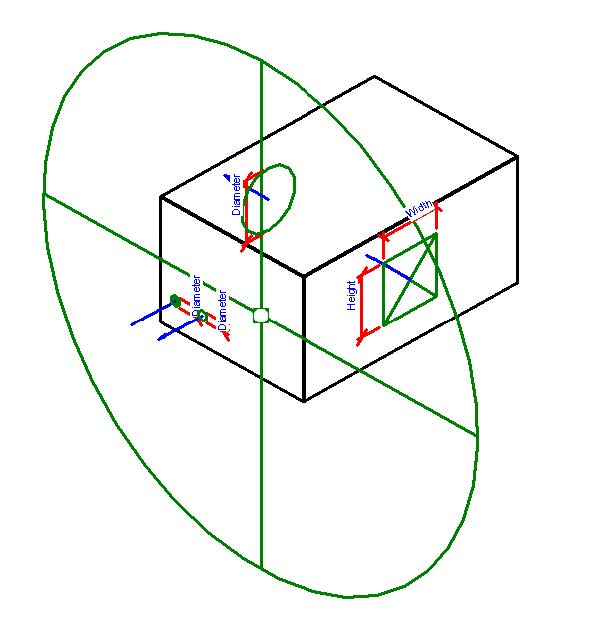
\includegraphics[width=0.7\linewidth]{./img/FanCoilUnit.jpg}
	\caption{Fan Coil Unit}
	\label{fig:fanCoilUnit}
\end{figure}




\begin{tabularx}{\textwidth}{ |c|X|c| }
	\hline
	\textbf{No.} & \textbf{Item} & \textbf{Details}\\
	\hline 
	1 & Length & 600 mm \\
	2 & Width & 400 mm \\
	3 & Height & 300 mm \\
	4 & Hydronic Supply & \diameter25 mm \\
	5 & Hydronic Return & \diameter25 mm \\
	6 & Single Pole Elec & 230V, PF 1.0, 600 VA \\
	7 & Duct In (Exhaust Air) & 150 mm x 150 mm \\
	8 & Duct Out (Supply Air) & \diameter150 \\
	\hline
\end{tabularx}

\subsection*{Upload Checklist}
\begin{tabular}{|l|l|l|}
	\hline
	\multicolumn{3}{| l |}{Part 1: Fan Coil Unit}\\
	\hline
	\textbf{Item} & \textbf{Format} & \textbf{Filename} \\
	\hline
	Revit File  & Revit Family File & RMEP04-***-00-ZZ-M3-M-Pr\_70\_65\_03\_29-401-A1-P01.rvt\\
	Revit File  & Revit Project File & RMEP04-***-00-ZZ-M3-M-401-A1-P01.rvt\\
	A1 Drawing  & Adobe pdf & RMEP04-***-00-ZZ-DR-M-401-A1-P01.pdf  \\
	\hline
\end{tabular}


\newpage


\section*{Part 2 - Generic Family Part}
In this section you are going to create a simple box shape with adjustable height, length and width. Once this is created you are going to create 3 types of the family and insert an instance of each into a Revit project. The family part should have three (3) reference planes named ‘Length’, ‘Width’ and ‘Height’. The family types should have the dimensions as shown in the table below.  Your completed Revit Family should be named \textbf{‘RMEP04-***-00-ZZ-M3-M-Pr\_20\_29\_08\_08-402-A1-P01.rfa’} and included in your submission folder.  Your completed Revit Project should be named ‘RMEP04-***-00-ZZ-M3-M-402-A1-P01.rvt’ and included in your submission folder. Fig: \ref{fig:GenericFamilyPart1}\\


\begin{tabularx}{\textwidth}{ |X|c|c|c| }
	\hline
	\textbf{Type Name} & Length & Width & Height \\
	\hline 
	Primo & 500 & 400 & 150\\
	Medio & 750 & 600 & 250\\
	Massimo & 1000 & 700 & 400\\
	\hline
\end{tabularx}


\begin{figure}[h]
	\centering
	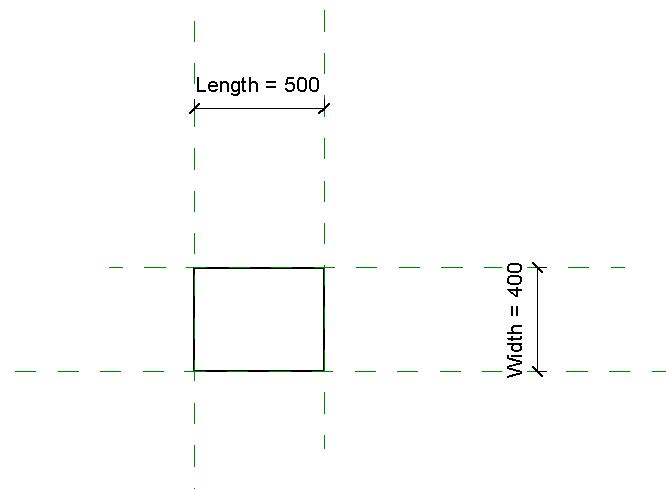
\includegraphics[width=0.7\linewidth]{./img/ParaBox1.jpg}
	\caption{Generic Family Part}
	\label{fig:GenericFamilyPart1}
\end{figure}


\begin{figure}[h]
	\centering
	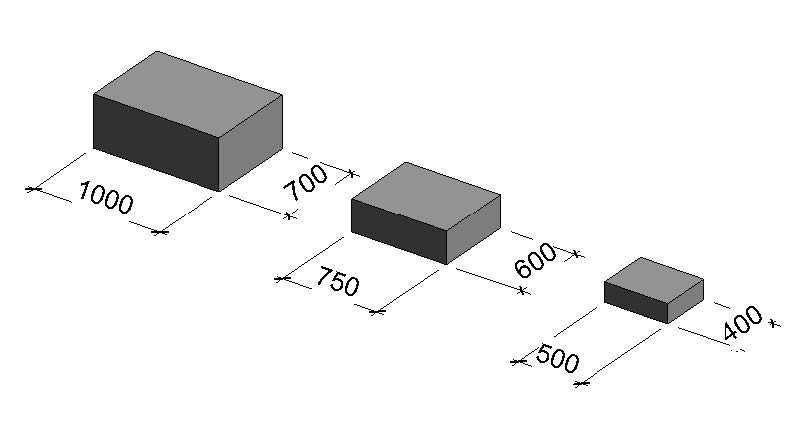
\includegraphics[width=0.7\linewidth]{./img/ParaBox2.jpg}
	\caption{Generic Family Part}
	\label{fig:GenericFamilyPart2}
\end{figure}


\subsection*{Upload Checklist}
\begin{tabular}{|l|l|l|}
	\hline
	\multicolumn{3}{| l |}{Part 2: Generic Family Part}\\
	\hline
	\textbf{Item} & \textbf{Format} & \textbf{Filename} \\
	\hline
	Revit File  & Revit Family File & RMEP04-***-00-ZZ-M3-M-Pr\_20\_29\_08\_08-402-A1-P01.rfa \\
	Revit File  & Revit Project File & RMEP04-***-00-ZZ-M3-M-402-A1-P01.rvt\\
	A1 Drawing  & Adobe pdf & RMEP04-***-00-ZZ-DR-M-402-A1-P01.pdf  \\
	\hline
\end{tabular}




\newpage

\section*{Part 3 - Auto generate Duct and Pipe Layouts}
Revit includes auto routing functionality for ducts and pipe. In this section you will create four (4) auto-routed duct layouts and two pipe layouts as shown below. Use the Revit Mechanical Template file to create your project. Your completed project file should be named \textbf{‘RMEP04-***-00-ZZ-M3-M-403-A1-P01.rvt’} and included in your submission folder.

\begin{figure}[h]
	\centering
	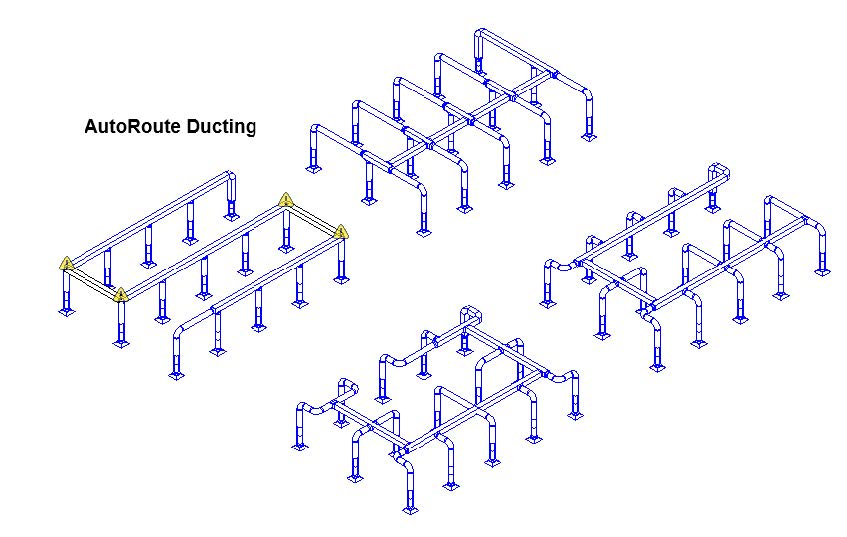
\includegraphics[width=0.9\linewidth]{./img/AutoRouteDuct.jpg}
	\caption{Revit Auto-routed Duct Layouts}
	\label{fig:AutorouteDuct}
\end{figure}


\begin{figure}[h]
	\centering
	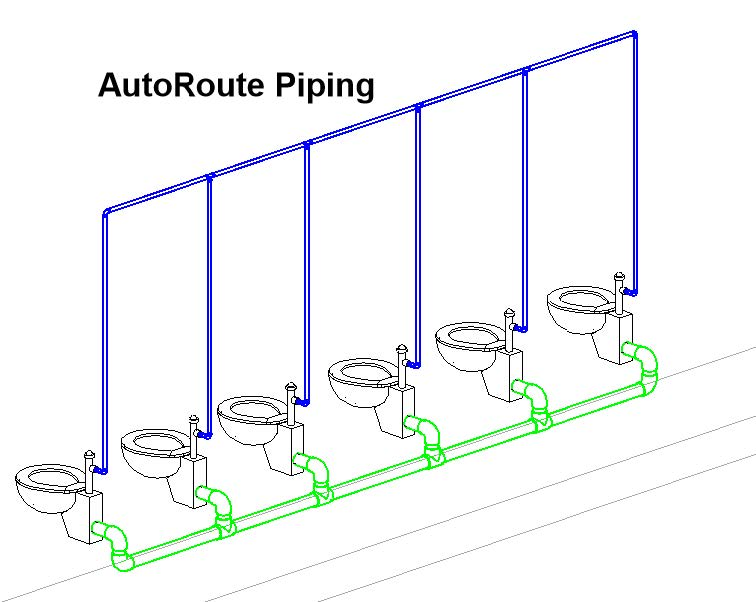
\includegraphics[width=0.7\linewidth]{./img/AutoRoutePipe.jpg}
	\caption{Revit Auto-routed Pipe Layouts}
	\label{fig:AutoroutePipe}
\end{figure}


\subsection*{Upload Checklist}
\begin{tabular}{|l|l|l|}
	\hline
	\multicolumn{3}{| l |}{Part 3:Auto Duct and Auto Pipe}\\
	\hline
	\textbf{Item} & \textbf{Format} & \textbf{Filename} \\
	\hline
	Revit File  & Revit Project File & RMEP04-***-00-ZZ-M3-M-403-A1-P01.rvt \\
	A1 Drawing  & Adobe pdf & RMEP04-***-00-ZZ-DR-M-403-A1-P01.pdf  \\
	\hline
\end{tabular}






\newpage

\section*{Part 4 (a) - Schedules with Images}
In this section you will create a furniture schedule that includes an image of the furniture item next to its information. You will use the architectural model provided for this section. Images to associate with each part have been provided in the asset pack for this assignment. You will need to apply the appropriate image to the Type Image parameter in the family editor. The completed table should be place on a Sheet view in the project file. Use the Save As function to create a new Revit project entitled \textbf{‘RMEP04-***-00-ZZ-M3-M-404-A1-P01.rvt’} and include this file in your assignment submission folder.
Revit Schedule with Images

\begin{figure}[h]
	\centering
	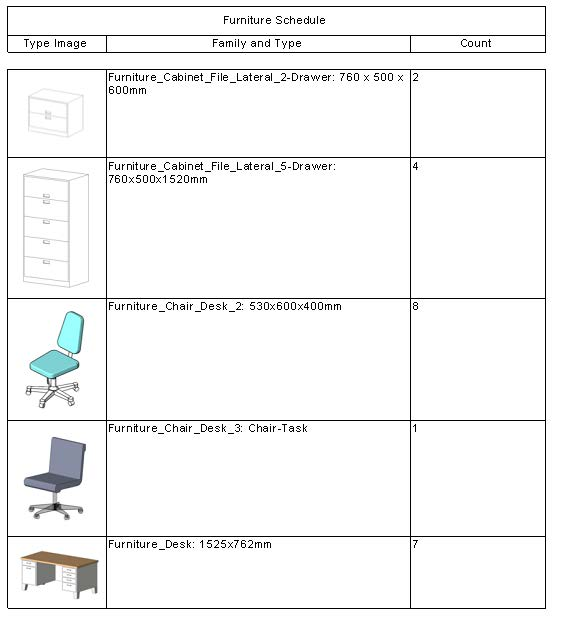
\includegraphics[width=0.7\linewidth]{./img/RevitSchedule.jpg}
	\caption{Revit Schedule with Images}
	\label{fig:ScheduleWithImages}
\end{figure}


\newpage


\section*{Part 4 (b) - Creating a Legend}
In this section you will create a 1:50 legend for the furniture in the architectural model provided in the asset pack. The headings are set to 5mm and the descriptions are set to 3.5mm. Unlike schedules, legends can be placed in multiple views, however there are some limitations. You are also required to add some simple dimensions to the images as shown below. Use the 'Save As' function to create a new Revit project entitled \textbf{‘RMEP04-***-00-ZZ-M3-M-404-A1-P01.rvt’} and include this file in your assignment submission folder.


\begin{figure}[h]
	\centering
	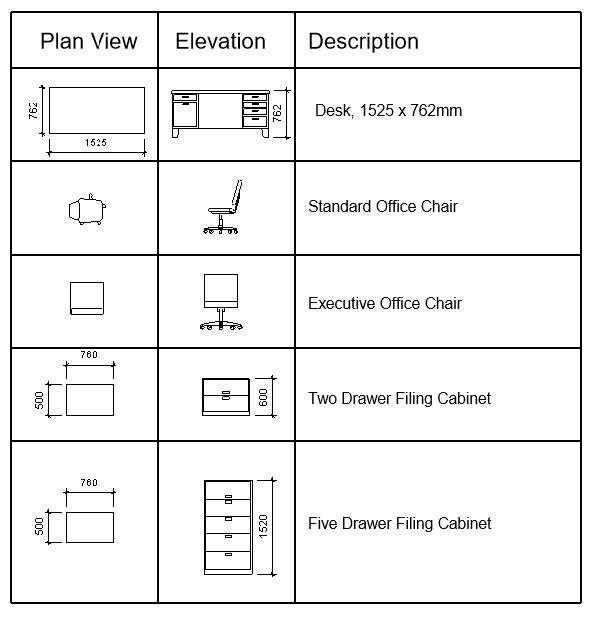
\includegraphics[width=0.7\linewidth]{./img/RevitLegend.jpg}
	\caption{Revit Legend with Images}
	\label{fig:RevitLegend}
\end{figure}





\subsection*{Upload Checklist}
\begin{tabular}{|l|l|l|}
	\hline
	\multicolumn{3}{| l |}{Part 4: Schedules and Legends}\\
	\hline
	\textbf{Item} & \textbf{Format} & \textbf{Filename} \\
	\hline
	Revit File  & Revit Project File & RMEP04-***-00-ZZ-M3-M-404-A1-P01.rvt \\
	A1 Drawing  & Adobe pdf & RMEP04-***-00-ZZ-DR-M-404-A1-P01.pdf  \\
	\hline
\end{tabular}



\newpage

\section*{Part 5 - Fabrication Parts}
In this section you will use the fabrication parts functionality in Revit to create the simple duct layout below. Create a new Revit project using the Mechanical template. Save your project file as \textbf{‘RMEP04-***-00-ZZ-M3-H-405-A1-P01.rvt’} and include it in your assignment submission.

\begin{figure}[h]
	\centering
	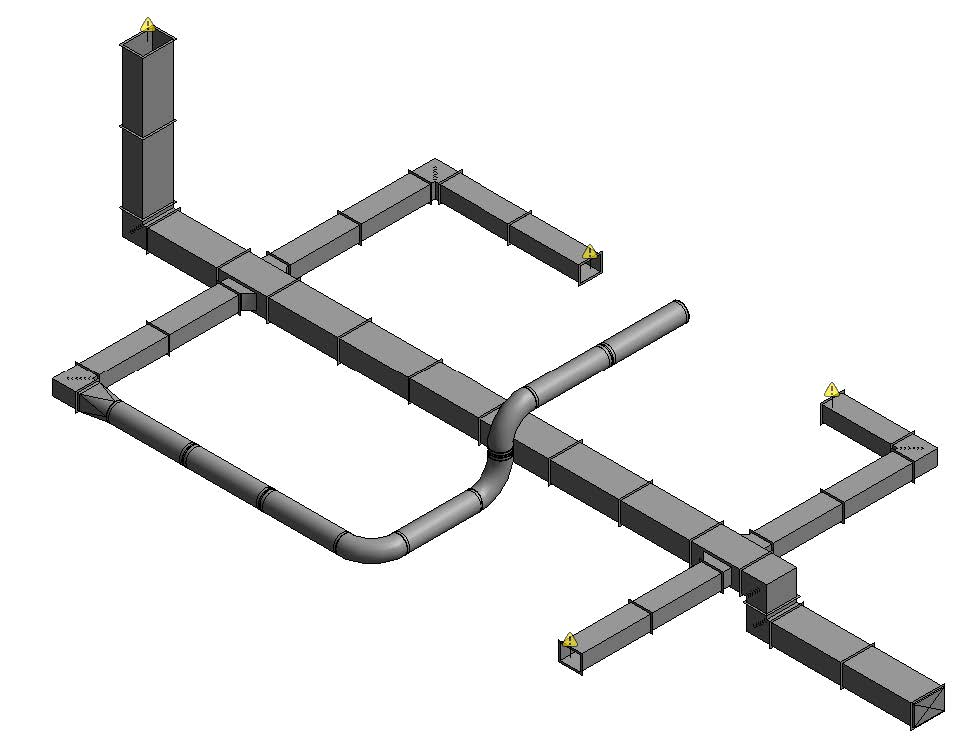
\includegraphics[width=0.7\linewidth]{./img/FabParts.jpg}
	\caption{Duct Layout using Fabrication Parts}
	\label{fig:FabParts}
\end{figure}


\begin{figure}[h]
	\centering
	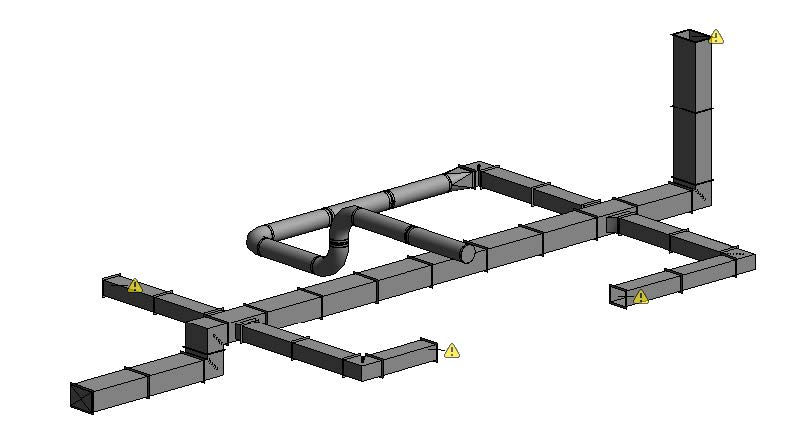
\includegraphics[width=0.7\linewidth]{./img/FabPartsReverse.jpg}
	\caption{Duct Layout using Fabrication Parts (Reverse Angle)}
	\label{fig:FabPartsReverse}
\end{figure}


\subsection*{Upload Checklist}
\begin{tabular}{|l|l|l|}
	\hline
	\multicolumn{3}{| l |}{Part 5: Fabrication Parts}\\
	\hline
	\textbf{Item} & \textbf{Format} & \textbf{Filename} \\
	\hline
	Revit File  & Revit Project File & RMEP04-***-00-ZZ-M3-H-405-A1-P01.rvt \\
	A1 Drawing  & Adobe pdf & RMEP04-***-00-ZZ-DR-H-405-A1-P01.pdf  \\
	\hline
	
\end{tabular}





\newpage

\section*{Upload Checklist}

\begin{tabular}{|l|l|l|}
	\hline
	
	\multicolumn{3}{| l |}{Part 1: Fan Coil Unit}\\
	\hline
	\textbf{Item} & \textbf{Format} & \textbf{Filename} \\
	\hline
	Revit File  & Revit Family File & RMEP04-***-00-ZZ-M3-M-Pr\_70\_65\_03\_29-401-A1-P01.rvt\\
	Revit File  & Revit Project File & RMEP04-***-00-ZZ-M3-M-401-A1-P01.rvt\\
	A1 Drawing  & Adobe pdf & RMEP04-***-00-ZZ-DR-M-401-A1-P01.pdf  \\
	\hline
	\hline
	\multicolumn{3}{| l |}{Part 2: Generic Family Part}\\
	\hline
	\textbf{Item} & \textbf{Format} & \textbf{Filename} \\
	\hline
	Revit File  & Revit Family File & RMEP04-***-00-ZZ-M3-M-Pr\_20\_29\_08\_08-402-A1-P01.rfa \\
	Revit File  & Revit Project File & RMEP04-***-00-ZZ-M3-M-402-A1-P01.rvt\\
	A1 Drawing  & Adobe pdf & RMEP04-***-00-ZZ-DR-M-402-A1-P01.pdf  \\
	\hline
	\hline
	\multicolumn{3}{| l |}{Part 3:Auto Duct and Auto Pipe}\\
	\hline
	\textbf{Item} & \textbf{Format} & \textbf{Filename} \\
	\hline
	Revit File  & Revit Project File & RMEP04-***-00-ZZ-M3-M-403-A1-P01.rvt \\
	A1 Drawing  & Adobe pdf & RMEP04-***-00-ZZ-DR-M-403-A1-P01.pdf  \\
	\hline
	\hline
	\multicolumn{3}{| l |}{Part 4: Schedules and Legends}\\
	\hline
	\textbf{Item} & \textbf{Format} & \textbf{Filename} \\
	\hline
	Revit File  & Revit Project File & RMEP04-***-00-ZZ-M3-M-404-A1-P01.rvt \\
	A1 Drawing  & Adobe pdf & RMEP04-***-00-ZZ-DR-M-404-A1-P01.pdf  \\
	\hline
	\hline
	\multicolumn{3}{| l |}{Part 5: Fabrication Parts}\\
	\hline
	\textbf{Item} & \textbf{Format} & \textbf{Filename} \\
	\hline
	Revit File  & Revit Project File & RMEP04-***-00-ZZ-M3-H-405-A1-P01.rvt \\
	A1 Drawing  & Adobe pdf & RMEP04-***-00-ZZ-DR-H-405-A1-P01.pdf  \\
	\hline

\end{tabular}



\end{document}